\documentclass[master]{thesis-uestc}

\title{面向方位失配问题的声波测井窜槽结构特征反演方法研究}{Research on Acoustic Logging Channeling Structure Feature Inversion under Azimuth Mismatch}
\author{TODO}{TODO}
\advisor{TODO}{TODO}
\school{TODO}{TODO}
\major{TODO}{TODO}
\studentnumber{TODO}
\classificationnumber{TODO}
\confidentiallevel{公开}
\udcnumber{TODO}
\setdate[submit]{TODO}
\setdate[oral]{TODO}
\setdate[confer]{TODO}

\newcommand{\placeholderfigure}[3]{%
\begin{figure}[htbp]
  \centering
  \fbox{%
    \begin{minipage}[c][0.25\textheight][c]{0.86\textwidth}
      \centering
      \vspace{0.5em}
      \textbf{图位占位}\\[0.8em]
      #1\\[0.8em]
      后续用手绘或重画图片替换，当前不插入真实图片。
      \vspace{0.5em}
    \end{minipage}
  }
  \caption{#2}
  \label{#3}
\end{figure}
}

\begin{document}

\makecover

\begin{chineseabstract}
固井质量评价是油气井完整性管理中的重要内容。水泥环窜槽可能造成层间流体连通和井筒完整性风险，因此需要利用测井资料对窜槽结构及其严重程度进行识别。阵列声波测井具有覆盖范围广、成本相对较低等优势，但其全波列响应受井眼环境、套管和水泥环共同影响，直接从低维声波指标中识别复杂窜槽结构存在困难。CAST 超声成像测井能够提供较高分辨率的环向声阻抗图像，可作为构造弱监督标签的重要依据。然而，在垂直井条件下，XSI 声波测井与 CAST 图像之间存在方位参考不可靠的问题，直接建立点对点方位监督容易引入错误标签。

针对上述问题，本文研究面向方位失配条件的声波测井窜槽结构特征反演方法。首先，将 XSI 全波列信号通过连续小波变换转换为多通道时频图，以保留声波响应的时间--频率联合特征。其次，基于 CAST 声阻抗阈值构造两类弱监督标签：一类为沿方位平均的一维窜槽百分比标签，作为直观的 fallback 对照；另一类为基于 severity map 的方位向 FFT magnitude 标签，通过丢弃相位降低对绝对方位匹配的依赖，作为本文方法主线。随后，采用 CWT-EfficientNetV2B0 回归模型学习 XSI 时频特征与 CAST 派生标签之间的映射关系，并在单井连续深度留出设置下进行验证。

实验结果表明，在 \texttt{array\_03} 单井 depth-heldout 条件下，EXP-008 的 FFT severity magnitude 标签路线取得测试 MAE 为 0.079025、RMSE 为 0.277019、R2 为 0.106634、Pearson 相关系数为 0.351950、Spearman 相关系数为 0.480519，说明该标签在连续深度留出测试段上具有一定可学习性。与简单基线相比，模型优于 train-mean 和 train-median baseline 的 MAE/RMSE/R2，并优于 zero baseline 的 RMSE/R2；但模型测试 MAE 未优于 zero baseline。EXP-007 的一维百分比标签在相同单井 depth-heldout 设置下可完成训练，但 R2 略为负，且同样未在 MAE 上优于 zero baseline。因此，本文将 EXP-008 作为方位失配问题下的主要方法探索，将 EXP-007 作为 fallback 与局限性对照。本文结果支持基于声波 CWT 特征与 CAST 弱监督标签的窜槽结构特征学习具有可行性，但现有证据仅限单井 depth-heldout，不代表多井泛化或工业部署性能。

\chinesekeyword{声波测井，水泥窜槽，方位失配，连续小波变换，FFT magnitude 标签，EfficientNet}
\end{chineseabstract}

\begin{englishabstract}
This thesis investigates a weakly supervised acoustic logging method for cement channeling structure feature inversion under azimuth mismatch. The English abstract is a draft and needs manual polishing after the Chinese manuscript and bibliography are finalized.

Cement channeling is an important risk factor for well integrity. Array sonic logging provides broad coverage and relatively low operational cost, while CAST ultrasonic imaging provides high-resolution azimuthal cement-bond information. However, direct azimuth-wise supervision between XSI sonic waveforms and CAST impedance images is unreliable in the studied vertical-well setting because the relative azimuth reference is not sufficiently stable. To avoid over-reliance on pointwise azimuth matching, this thesis constructs weak supervision labels from CAST impedance maps and learns their relationship with XSI continuous-wavelet-transform time-frequency representations.

Two label routes are studied. The first route constructs a one-dimensional percentage label by azimuthal averaging and is used as a fallback comparison. The second route transforms CAST impedance into a severity map and then applies an azimuthal FFT magnitude transform. Since circular shifts mainly affect FFT phase while preserving magnitude, the FFT magnitude label reduces the dependence on absolute azimuth alignment and is used as the main method route. An EfficientNetV2B0-based regression model is trained with explicit train/validation/test TFRecords generated by a continuous depth-heldout split.

Under a single-well \texttt{array\_03} depth-heldout setting, the EXP-008 FFT severity magnitude route achieves a test MAE of 0.079025, RMSE of 0.277019, R2 of 0.106634, Pearson correlation of 0.351950, and Spearman correlation of 0.480519 on 423 test samples. These results indicate metric-qualified learnability, but the model does not outperform the zero baseline in MAE. The EXP-007 percentage-label fallback is trainable but does not provide stronger evidence than EXP-008. Therefore, the thesis presents the FFT severity magnitude label as a feasible exploration for azimuth-mismatch-aware weak supervision, while explicitly limiting the conclusion to single-well depth-heldout evidence rather than multi-well generalization or industrial deployment performance.

\englishkeyword{Acoustic logging, cement channeling, azimuth mismatch, continuous wavelet transform, FFT magnitude label, EfficientNet}
\end{englishabstract}

\thesistableofcontents

\chapter{绪\hspace{6pt}论}

\section{研究背景与意义}

固井质量评价是油气井建井和长期生产过程中的关键环节。水泥环承担封隔地层、保护套管和维持井筒完整性的作用。当水泥环与套管或地层之间存在胶结不良、微环空或窜槽时，可能造成层间流体连通、产量下降以及井筒完整性风险。因此，利用测井资料对水泥胶结状态进行识别和评价具有明确的工程意义。

声波测井和超声成像测井是固井质量评价中的重要资料来源。声波测井具有覆盖范围广、成本相对较低、适合全井段普查等优势，但其全波列信号受到多种模式波、套管波、地层波和井眼环境的共同影响，传统的低维幅度或能量指标难以充分表达复杂窜槽结构。CAST 等超声成像测井能够提供较高分辨率的环向声阻抗图像，在窜槽位置和方位结构方面具有更直观的信息。若能利用 CAST 图像构造监督信号，并从 XSI 声波全波列中学习窜槽相关结构，将有助于探索声波资料在固井质量评价中的更充分利用。

然而，声波测井与超声成像测井并非天然对齐。二者的测量物理、采样分辨率、深度采样方式和方位参考均存在差异。尤其在本文所关注的垂直井场景中，XSI 与 CAST 的相对方位参考不稳定，旧实验未能支持可靠的点对点方位监督。因此，本文不将 CAST 环向像素直接作为 XSI 方位通道的逐点标签，而是围绕方位失配问题构造弱监督标签，研究声波 CWT 时频特征与 CAST 派生窜槽结构特征之间的可学习关系。

\placeholderfigure{固井质量、水泥环、窜槽通道、套管和地层之间关系的手绘示意。}{固井质量评价与窜槽问题示意图。该图用于说明水泥环窜槽可能导致层间连通和井筒完整性风险，不包含实验性能结论。}{fig:cement-channeling}

\section{固井质量评价与窜槽识别研究现状}

传统固井质量评价通常依赖声波幅度、变密度测井、声波全波列特征以及超声成像资料等信息。声波幅度类指标解释简单，但容易受到套管、地层和仪器条件影响；全波列资料包含更丰富的传播和散射信息，但人工解释和低维特征提取难以完整利用其时频结构。超声成像资料能够提供更直观的环向图像，对识别水泥环局部缺陷具有优势，但其作业成本、测量条件和覆盖范围也限制了其作为唯一评价手段的使用。

近年来，基于机器学习和深度学习的方法被用于测井解释和图像识别任务。对于固井质量评价问题，深度模型可以从高维波形或时频图中提取非线性特征。但模型性能依赖可靠标签，若标签构造没有处理好多源测井之间的空间、深度或方位不一致，就可能得到表面上较高但实质上受泄漏或错配影响的指标。因此，本文将标签工程和样本划分作为方法设计的核心部分，而不是仅仅比较模型主干。

\section{声波测井与超声成像测井方法概述}

XSI 阵列声波测井记录多接收器、多方位通道的全波列响应。该类数据包含不同传播模式在时间和频率上的叠加，适合通过连续小波变换进行时频展开。CAST 超声成像测井则以环向扫描方式得到声阻抗图像，可用于描述水泥胶结状态的方位分布。本文将 CAST 声阻抗阈值化后构造 severity map，并进一步生成一维 percentage label 或方位向 FFT magnitude label。

\placeholderfigure{左侧为 XSI 多通道声波波形或 CWT 时频图，右侧为 CAST 环向 Zc 图像，中间标注二者数据形态和分辨率差异。}{XSI 与 CAST 测井响应差异示意图。该图用于说明声波时频响应与 CAST 环向成像之间的数据形态差异。}{fig:xsi-cast-difference}

\section{深度学习在测井解释中的应用现状}

深度学习模型能够从高维输入中自动提取层级特征，已被广泛用于图像识别、序列分析和地球物理数据解释等任务。对于声波全波列，直接使用原始时间序列可能难以显式刻画瞬态频率变化；连续小波变换将一维信号映射到二维时频域，使卷积神经网络能够处理局部时间--频率结构。EfficientNetV2B0 作为高效卷积网络主干，可用于从 CWT 图像中提取特征并执行回归任务。

需要强调的是，本文不以模型结构复杂度作为主要创新点。本文重点在于：在 XSI 与 CAST 方位失配条件下，如何构造更稳健的 CAST 派生弱监督标签，并用 single-well depth-heldout 实验检验其可学习性。

\section{现有研究存在的问题}

结合旧项目实验与最终证据冻结，本文面对的主要问题包括：

\begin{enumerate}
  \item XSI 与 CAST 的方位参考不可靠，直接点对点方位监督不适合作为主线。
  \item 一维 percentage label 直观但会丢弃方位结构，且标签稀疏时 zero baseline 在 MAE 上很强。
  \item FFT magnitude label 能降低对绝对方位的依赖，但丢弃相位后不再保留完整方位位置信息。
  \item 连续深度样本之间具有相似性，random split 可能带来相邻深度泄漏风险。
  \item 当前最终证据仅覆盖 \texttt{array\_03} 单井 depth-heldout，不支持多井泛化或工业部署结论。
\end{enumerate}

\section{本文研究内容与技术路线}

本文围绕方位失配条件下的声波测井窜槽结构特征反演开展研究。主要内容包括：构建 XSI CWT 时频输入；基于 CAST Zc 构造 severity map、一维 percentage label 和方位向 FFT magnitude label；建立 CWT-EfficientNetV2B0 回归模型；区分 random split 探索实验与 single-well depth-heldout 验证实验；分析 EXP-008 主线结果、EXP-007 fallback 结果及 EXP-006 exploratory baseline。

\placeholderfigure{从 XSI 波形、CWT、CAST Zc、severity map、FFT magnitude label、EfficientNet 回归、depth-heldout 验证到误差分析的流程图。}{本文技术路线图。该图展示本文从数据构建、标签构造到模型训练和结果审计的整体流程。}{fig:technical-route}

\section{本文组织结构}

第 1 章介绍研究背景、意义和本文研究内容。第 2 章说明 XSI 与 CAST 数据基础，并分析方位失配和样本划分问题。第 3 章提出旋转不变标签构建和 CWT-EfficientNetV2B0 回归方法。第 4 章给出 random split 探索实验、EXP-008 主实验、EXP-007 fallback 实验和 EXP-006 baseline 的结果分析。第 5 章讨论标签设计意义、zero baseline MAE 问题、误差来源和单井泛化限制。第 6 章总结全文并给出后续工作方向。

\chapter{数据基础与问题分析}

\section{数据来源与总体说明}

本文研究数据来源于与美国哈里伯顿公司开展的横向合作项目。本研究基于哈里伯顿公司提供的同一井段 XSI 阵列声波测井数据、CAST 超声成像测井数据和工具姿态相关数据，分析声波响应与套管外水泥环状态之间的关系。为避免披露与研究目标无关的信息，本文只给出数据结构、井段范围和必要的处理参数，不公开井名、地理位置及生产信息。

研究井段为 2732--4132~ft。主要数据包括：XSI 多接收器全波列、CAST 声阻抗矩阵，以及与 XSI 深度对应的 Relative Bearing 和 Inclination。XSI、CAST 和姿态数据分别具有不同的采样间隔和记录顺序，本研究先核验各自深度轴，再在 0.1~ft 派生深度网格上构造样本。该网格是本研究的数据处理参数，不是仪器原始采样分辨率。

数据核验采用项目 MAT 文件、处理代码、配置文件、汇报材料和公开工具论文相互印证。公开工具论文用于说明接收器几何和一般测量原理，项目文件用于确定本研究实际使用的数组维度和处理参数。二者发生差异时，以“仪器结构”和“本文数据子集”分别表述，避免把处理窗口写成仪器能力。

\begin{table}[htbp]
  \centering
  \small
  \setlength{\tabcolsep}{4pt}
  \caption{本文使用的主要数据及其原始组织}
  \label{tab:data-overview}
  \begin{tabular}{p{0.20\textwidth}p{0.25\textwidth}p{0.22\textwidth}p{0.23\textwidth}}
    \toprule
    数据 & 主要变量 & 原始数组 & 本文用途 \\
    \midrule
    XSI 第 3 接收环 & Depth、Tad、SideA--SideH & 每个侧向波形矩阵为 $1024\times7108$ & 构造 8 通道 CWT 输入 \\
    CAST & Depth、$Z_c$ & $Z_c$ 为 $180\times24750$ & 构造深度--方位参考标签 \\
    工具姿态 & Depth、Inc、RelBearing & 三个长度均为 13508 的向量 & 分析井斜与相对方位可靠性 \\
    \bottomrule
  \end{tabular}
\end{table}

在目标井段内，XSI 第 3 接收环共有 2852 条深度记录，其中 2846 个深度值唯一；CAST 对应 9884 个深度记录；姿态数据对应 5549 条记录。数据量差异来自工具采样方式，不代表一一对应关系。最终回归实验按共同有效范围和样本窗口形成 2842 个候选样本，其中 19 个位于划分缓冲区，不参与训练、验证或测试。

\section{XSI 声波测井数据结构}

\subsection{工具几何与数据子集}

XSI 类超宽带阵列声波工具通过多个单极和偶极声源激发井内波场，并由轴向、周向分布的接收器记录波形。公开工具论文给出的接收段包含 13 个轴向接收环，每环 8 个接收器沿周向等间隔布置，共 104 个接收器\cite{Sun2016UltrabroadbandAcoustic}。13 个接收环提供不同源距，8 个周向单元提供工具坐标系内的方位采样。这里的“$13\times8$”描述仪器接收器几何，不等于本文模型输入维度。

项目数据按接收环拆分。本文使用第 3 接收环，对应 SideA 至 SideH 共 8 个周向通道；其余接收环不进入本轮模型。项目配置给出的 13 个接收环相对源偏移从 3~ft 到 $-3$~ft，以 0.5~ft 递减，第 3 接收环偏移为 2~ft。接收器字母只表示工具内部的周向编号。除非同时知道工具姿态和每个字母相对参考方向的定义，SideA 不能直接解释为北向、井眼高边或 CAST 图像零点\cite{Che2014PhasedArcReception,Che2017AzimuthalReceiver}。

\subsection{时间采样与分析窗口}

第 3 接收环每个侧向通道的原始波形长度为 1024 点，存储类型为 32 位整数。项目数据采样率为 100~kHz，对应采样间隔为 10~$\mu$s，单条原始波形记录时长约为 10.24~ms。本文仅选取每条波形的前 400 点，即约 4~ms，用于覆盖研究所关注的早期声波响应。400 点是本文的预处理窗口，不能表述为仪器只能采集 400 点。

100~kHz 采样率对应 50~kHz 的奈奎斯特频率，但奈奎斯特频率不等于仪器换能器的有效响应范围。本文 CWT 采用 1--30~kHz 的分析频带，该范围由项目处理配置确定。公开工具论文展示了不同发射模式和处理频带\cite{Sun2016UltrabroadbandAcoustic}，但本文不据此推定本项目仪器的原始带宽；1--30~kHz 仅表示本文选取的 CWT 分析频带。

\subsection{深度轴、异常值与张量维度}

XSI 第 3 接收环在目标井段的唯一深度间隔中位数约为 0.493~ft，存在 9 个重复深度以及少量局部顺序变化。处理时先按深度排序、合并重复索引，再映射到统一网格。8 个通道的原始矩阵均为有限整数，未发现 NaN 或 Inf。原始 XSI 波形中存在少量达到有符号 24 位数字量程上下限的采样点，其数值分别为 $-8388608=-2^{23}$ 和 $8388607=2^{23}-1$，表现为局部采集饱和或数字削顶。模型实际输入范围内共检测到 156 个端点采样值，其中下限值 109 个、上限值 47 个，涉及 75 条深度记录。没有证据表明这些端点是缺测编码。

历史预处理没有对上述端点值执行专门的掩膜、替换或人工裁剪，而是将前 400 点直接送入 1~kHz 四阶零相位高通。滤波结果保持有限，但线性滤波不等同于对削顶波形的恢复。由于端点数量在整体输入数据中极少，经项目数据核查，其对模型总体实验结果的影响可以忽略；本文仍将其作为原始采集数据的质量现象予以说明，不将“影响可以忽略”表述为“完全没有影响”。

单个深度样本经 1~kHz 四阶零相位高通、前 400 点截取和复 Morlet CWT 后，每个通道形成 $150\times400$ 的时间--频率图。8 个周向通道堆叠后，模型输入张量为
\begin{equation}
  \mathbf{X}\in\mathbb{R}^{150\times400\times8},
  \label{eq:xsi-input-shape}
\end{equation}
其中 150 为尺度或频率采样数，400 为时间采样数，8 为第 3 接收环的周向通道数。

\begin{table}[htbp]
  \centering
  \caption{XSI 原始参数与本文处理参数的区分}
  \label{tab:xsi-parameters}
  \begin{tabular}{p{0.32\textwidth}p{0.25\textwidth}p{0.32\textwidth}}
    \toprule
    项目 & 核验值 & 属性 \\
    \midrule
    接收器几何 & 13 环，每环 8 个接收器 & 公开工具结构 \\
    本文接收环 & 第 3 环，SideA--SideH & 研究数据子集 \\
    原始波形长度 & 1024 点 & 项目 MAT 文件 \\
    时间采样间隔 & 10~$\mu$s & 项目数据采样参数 \\
    本文时间窗 & 前 400 点，4.00~ms & 预处理参数 \\
    采样率/奈奎斯特频率 & 100/50~kHz & 项目配置/数学上限 \\
    本文 CWT 频带 & 1--30~kHz & 特征提取参数 \\
    CWT 输入维度 & $150\times400\times8$ & 模型输入 \\
    \bottomrule
  \end{tabular}
\end{table}

\section{CAST 超声成像数据结构}

\subsection{测量原理与矩阵组织}

CAST 数据以超声脉冲回波测量为基础。换能器向套管内壁发射脉冲，回波的到达、幅度和共振衰减受套管厚度、井液以及套管后介质影响。通过周向扫描，可将套管后介质的等效声阻抗按深度和方位排列为图像。脉冲回波、弯曲波和传统声波胶结测量对不同波模态敏感，解释时应结合其适用条件\cite{Froelich1982CementEvaluation,Froelich2008MultimodeCement,Wang2016AcousticCementMethods}。

声阻抗通常定义为
\begin{equation}
  Z=\rho c,
  \label{eq:acoustic-impedance}
\end{equation}
其中 $\rho$ 为介质密度，$c$ 为声速。套管与套管后介质的阻抗和界面耦合共同影响回波。低声阻抗响应可能与液体通道或胶结较差有关，但不能仅凭一个像素断言其对应真实窜槽。

CAST 数据中的 $Z_c$ 表示套管外介质的声阻抗，单位为 MRayl。项目 \texttt{CAST.mat} 中的 $Z_c$ 矩阵为 $180\times24750$，第一维为周向采样，第二维为深度。每个深度位置包含 180 个等角度方位采样点，相邻方位间隔为 $2^\circ$，完整覆盖井周 $360^\circ$。深度从约 2395.445~ft 延伸到 5804.337~ft，在目标井段内有 9884 个记录，深度间隔中位数约为 0.142~ft。完整周向覆盖和采样间隔已经确认，但现有数据不包含可将 CAST 方位零点唯一转换到 XSI 通道零点的共同参考信息。

\subsection{数值质量与派生标签}

$Z_c$ 矩阵中的 4,455,000 个元素均为有限数值，没有 NaN 或 Inf；全数据中有 14 个负值。根据项目事实，负声阻抗缺乏合理物理意义，应视为无效值。历史预处理代码并未对它们显式掩膜、替换、裁剪或插值修复，而是先按深度对整幅 $Z_c$ 线性插值。数据复核表明，这 14 个原始负值分布于 2469.003--2504.845~ft 和 4898.053~ft，全部位于本文 2732--4132~ft 目标井段之外；目标井段原始数据和 0.1~ft 插值网格中均没有负值。因此，这些无效值没有进入本文的一维占比标签或 FFT 幅值标签，也没有影响已完成实验指标。该结论来自位置与代码链核查，不能改写成“历史代码已经执行负值掩膜”。

根据美国哈里伯顿公司在本项目 CAST 成像解释中采用的数据判别约定，本文选取 $Z_c=2.5~\mathrm{MRayl}$ 作为参考阈值。该数值并非本文自行提出或通过优化得到，也不是适用于所有工具、井况和水泥体系的普适行业标准。由该阈值得到的严重度和结构标签属于参考工具成像结果的派生表征，既不是直接测量得到的绝对真实标签，也不能解释为绝对窜槽宽度或缺陷体积。

\section{XSI--CAST 方位失配问题分析}

\subsection{需要区分的坐标量}

方位关系分析中需要区分六类量：

\begin{enumerate}
  \item 仪器方位：工具坐标系相对某一外部参考方向的转角；
  \item 接收器编号：SideA--SideH 在工具圆周上的相对位置；
  \item 井眼高边：倾斜井眼横截面中重力意义上的上方方向；
  \item Relative Bearing：工具某参考轴相对于指定参考方向的周向角；
  \item Inclination：井眼或工具轴相对铅垂方向的倾角；
  \item CAST 与 XSI 方位零点：两套数据周向索引各自的起始方向。
\end{enumerate}

方位阵列文献通常在接收器几何和参考方向已知时讨论入射方向或窜槽方位\cite{Che2014PhasedArcReception,Che2017AzimuthalReceiver,Zuo2020AzimuthCement}。本文虽然知道八个 XSI 通道以 $45^\circ$ 相对间隔布置，但缺少 CAST 零点和 XSI 工具参考轴之间的唯一对应。相对间隔已知不等于绝对起点已知。

\subsection{Inclination 数据分析}

目标井段 Inclination 的最小值为 $0.1349^\circ$，最大值为 $2.2879^\circ$，均值为 $0.5218^\circ$，中位数为 $0.4705^\circ$；5\%--95\% 分位范围约为 $0.2097^\circ$--$1.1975^\circ$。这说明研究井段总体接近直井。在接近铅垂时，井眼高边方向对微小姿态和测量噪声更敏感。

Inclination 是工具轴相对铅垂方向的倾角大小，不包含绕工具轴旋转的方向信息。即使倾角测量完全可靠，也不能由一个标量倾角推导 XSI 方位零点相对 CAST 零点的旋转。因此，Inclination 不能直接作为方位校正角。

\begin{figure}[htbp]
  \centering
  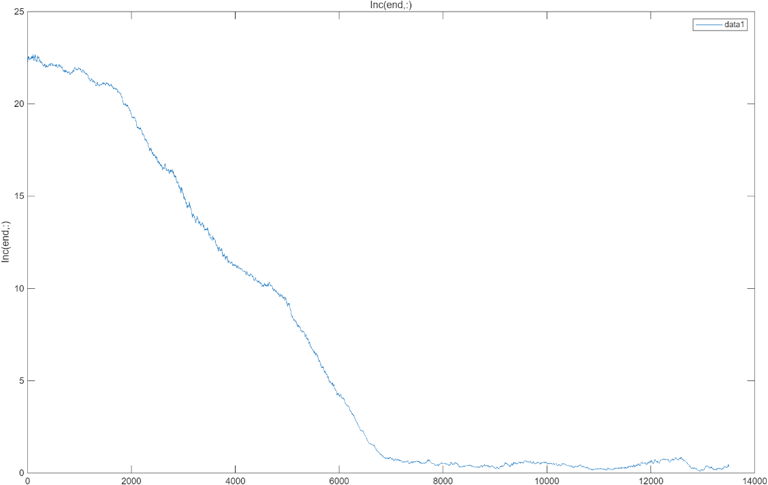
\includegraphics[width=0.78\textwidth]{figures/revision/inclination.png}
  \caption{Inclination 随记录索引的变化。目标井段总体接近直井}
  \label{fig:inclination}
\end{figure}

\subsection{Relative Bearing 数据分析}

在 2732--4132~ft 目标井段内，Relative Bearing 范围约为 $1.85^\circ$--$357.82^\circ$。按圆周差计算，相邻记录绝对变化的中位数为 $5.156^\circ$，95\% 分位为 $28.639^\circ$，99\% 分位为 $64.611^\circ$，最大值为 $178.563^\circ$；其中 111 次变化超过 $45^\circ$，23 次超过 $90^\circ$。图 \ref{fig:relative-bearing} 显示，接近直井的区间存在明显跳变，而井斜增大后的区间更平滑。该现象与项目汇报中“近直井段 Relative Bearing 可靠性较低”的记录一致。

\begin{figure}[htbp]
  \centering
  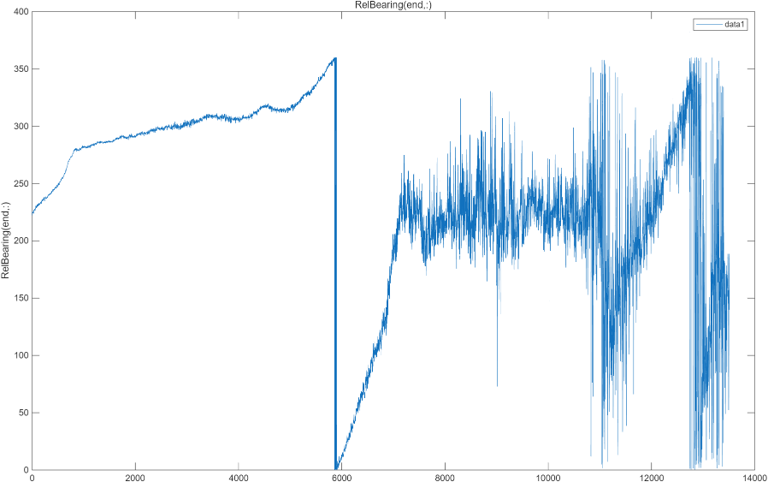
\includegraphics[width=0.78\textwidth]{figures/revision/relative_bearing.png}
  \caption{Relative Bearing 随记录索引的变化。接近直井区间存在较多周向跳变}
  \label{fig:relative-bearing}
\end{figure}

然而，当前 MAT 文件没有给出 Relative Bearing 的正式参考方向定义，也没有给出 CAST 方位零点。仅凭曲线连续性无法判断某一数值对应磁北、井眼高边、工具面还是其他处理约定。受现有工具姿态元数据和方位基准信息限制，本文无法建立两类测井数据绝对方位零点之间的唯一转换关系。

\subsection{深度差异与标签误差}

XSI、CAST 和姿态数据的原始深度采样分别约为 0.493、0.142 和 0.25~ft 的量级，并存在局部重复、重排或间隔变化。深度插值可以把三类数据映射到共同网格，却不能补充缺失的方位零点。若在没有绝对零点转换的条件下，把 CAST 第 $j$ 个方位像素直接赋给 XSI 第 $j$ 个通道，同一物理结构可能因未知循环移位而对应不同标签。这种误差不是增加样本量即可自动消除的随机噪声，而是与工具姿态相关的系统性标签不一致。

本文大部分实验使用 2732--4132~ft 井段。该井段 Inclination 中位数仅为 $0.4705^\circ$，整体接近直井；与此同时，Relative Bearing 呈现频繁且幅度较大的跳变，Inclination 又只描述井斜大小，不能充当绕工具轴的旋转校正角。结合 XSI 与 CAST 绝对方位零点之间缺少唯一转换关系这一事实，本文不把 CAST 的绝对方位位置作为监督目标，也不建立未经证据支持的绝对角度公式。

对 CAST 的 180 点完整周向序列，未知方位零点差异在离散表示上建模为循环平移。第三章沿方位维进行离散傅里叶变换并使用幅值：循环移位改变相位而不改变幅值，从而降低未知方位移位的影响。该标签保留环向结构的频率组成，但舍弃绝对方位位置和相位信息；它不能恢复窜槽的绝对方位，也不能替代可靠的工具姿态配准。

\section{相邻深度相关性与验证边界}

声波和 CAST 标签均由连续深度窗口构造，相邻样本可能共享相近地层、套管条件和重叠窗口。对这类结构化数据进行随机划分，训练集与测试集容易包含邻近深度，从而低估预测误差\cite{Roberts2017CrossValidation,Valavi2019BlockCV}。本文将随机样本划分用于先导可学习性检验，将主要回归结论建立在单井深度区间隔离划分上。

严格划分中，训练集为 1984 个样本，深度范围 2732.440--3715.853~ft；验证集为 416 个样本，范围 3721.119--3917.685~ft；测试集为 423 个样本，范围 3922.785--4129.744~ft。相邻集合之间设置 5~ft 缓冲区，共排除 19 个样本。三个集合的深度键无交集。该设置提高了同井验证的严格程度，但仍不能代替跨井验证。

\section{本章小结}

本章从项目文件、已确认项目事实和公开工具论文核验了 XSI、CAST 与姿态数据。XSI 工具具有 13 环、每环 8 个接收器的结构，共 104 个接收通道，而本文仅使用第 3 接收环的 8 通道、前 400 点波形；少量 24 位端点削顶对总体实验结果的影响可以忽略，但仍作为数据质量现象保留说明。CAST 声阻抗单位为 MRayl，由 180 个按 $2^\circ$ 等间隔覆盖完整井周的方位点和不规则深度轴组成，其 $2.5~\mathrm{MRayl}$ 阈值是哈里伯顿公司在本项目成像解释中采用的项目约定。Inclination 只表示井斜大小，Relative Bearing 在目标近直井段存在频繁跳变，且两类工具缺少可相互转换的绝对方位零点。上述事实构成不使用绝对方位位置监督、采用方位向 FFT 幅值标签和深度区间隔离验证的直接依据。

\chapter{旋转不变标签构建与模型方法}

\section{方法总体框架}

本文方法框架由三部分组成：第一，基于 XSI 全波列构建 CWT 时频输入；第二，基于 CAST Zc 构建弱监督标签，包括一维 percentage label 和 FFT severity magnitude label；第三，采用 EfficientNetV2B0 回归模型学习 CWT 输入到标签空间的映射。该框架的核心不是直接恢复 CAST 的绝对方位图像，而是在方位失配条件下学习与窜槽结构相关的弱监督表征。

\placeholderfigure{XSI CWT 输入、CAST 标签构建、EfficientNet 回归、depth-heldout 评估和误差分析模块。}{本文方法总体框架图。该图展示本文从多源数据到弱监督回归模型的整体方法。}{fig:method-framework}

\section{1D percentage label 构建}

一维 percentage label 是本文的 fallback 标签路线。其构建过程首先根据 CAST Zc 阈值生成二值窜槽掩膜：
\begin{equation}
  m(d,\theta)=
  \begin{cases}
  1, & Z_c(d,\theta)<2.5,\\
  0, & Z_c(d,\theta)\ge 2.5.
  \end{cases}
  \label{eq:binary-mask}
\end{equation}
随后沿方位方向求平均，得到深度方向的一维窜槽比例：
\begin{equation}
  p(d)=\frac{1}{N_\theta}\sum_{\theta=1}^{N_\theta} m(d,\theta).
  \label{eq:percentage-label}
\end{equation}

该标签的优点是含义直观，避免了 XSI 与 CAST 的方位点对点匹配；缺点是完全丢弃方位结构，并在标签稀疏时使 zero baseline 在 MAE 上具有较强竞争力。因此，本文将其用于 EXP-007 fallback/limitation comparison，而不作为最终方法创新主线。

\placeholderfigure{CAST Zc 到二值窜槽掩膜，再沿方位平均得到一维百分比剖面。}{1D percentage label 构建流程图。该图说明一维标签如何降低方位对齐要求，同时也丢弃方位结构。}{fig:percentage-label}

\section{severity map 构建}

为了保留窜槽严重度而非仅使用二值掩膜，本文采用式 \ref{eq:severity} 将 CAST Zc 转换为 severity map。与二值标签相比，severity map 对低声阻抗异常区域赋予连续强度，有助于描述窜槽严重度和环向分布。

\placeholderfigure{CAST Zc 图像、阈值函数和 severity map 的对应关系。}{severity map 构建示意图。该图说明 CAST 声阻抗如何转换为连续严重度标签。}{fig:severity-construction}

\section{基于方位向 FFT magnitude 的旋转不变标签}

对于每个深度位置 $d$，将 severity map 沿方位方向记为序列 $s_d(\theta)$。对其进行离散傅里叶变换：
\begin{equation}
  S_d(k)=\sum_{n=0}^{N_\theta-1}s_d(n)\exp\left(-j2\pi kn/N_\theta\right),
  \label{eq:fft}
\end{equation}
并取幅度谱作为标签：
\begin{equation}
  y_d(k)=|S_d(k)|.
  \label{eq:fft-mag}
\end{equation}

若方位序列发生循环平移，傅里叶变换的相位将发生变化，而幅度保持不变。因此，FFT magnitude 标签能够降低对绝对方位匹配的依赖。需要强调的是，该标签并不保留完整方位位置信息，也不能表述为完全解决方位失配问题。它的作用是在保留部分环向结构频率信息的同时，避免将不可靠相位作为监督目标。

\placeholderfigure{同一环向 severity 序列旋转前后，FFT phase 改变而 magnitude 基本保持的示意。}{方位旋转对 FFT phase 与 magnitude 的影响示意图。该图用于说明 FFT magnitude 标签的旋转不变性来源。}{fig:fft-invariance}

\placeholderfigure{CAST Zc、severity map、方位向 FFT、magnitude 截取和最终回归标签形状。}{severity map 到 FFT magnitude label 的构建流程图。该图对应 EXP-008 主线标签路线。}{fig:fft-label}

\section{XSI 波形 CWT 时频图构建}

声波全波列是典型非平稳信号。本文采用连续小波变换将每个通道的一维时间序列转换为二维时频图：
\begin{equation}
  W_x(a,b)=\frac{1}{\sqrt{a}}\int x(t)\psi^\ast\left(\frac{t-b}{a}\right)\mathrm{d}t,
  \label{eq:cwt}
\end{equation}
其中 $a$ 为尺度，$b$ 为时间平移，$\psi$ 为小波基函数。参考材料和代码证据表明，CWT 输入可表述为多通道时频张量，用于 EfficientNet 图像回归模型。

\placeholderfigure{多通道 XSI 波形分别进行 CWT，形成可输入卷积模型的时频张量。}{XSI 波形到 CWT 时频图的转换示意图。该图用于说明模型输入特征的构建方式。}{fig:cwt-construction}

\section{CWT-EfficientNetV2B0 回归模型}

本文采用 EfficientNetV2B0 作为 CWT 图像特征提取主干。由于 CWT 输入包含多个声波通道，模型前端可使用 $1\times1$ 卷积进行通道适配，随后经过 EfficientNetV2B0、全局平均池化、Dropout 和全连接回归头输出目标标签。对于 EXP-008，输出为 FFT severity magnitude 标签；对于 EXP-007，输出为一维 percentage profile 标签。

\placeholderfigure{CWT 多通道输入、1x1 通道适配、EfficientNetV2B0、Global Average Pooling、Dropout、Dense 回归头。}{CWT-EfficientNetV2B0 回归模型结构图。该图用于说明本文主线模型结构，不作为性能证明。}{fig:efficientnet-architecture}

\section{训练目标与评价指标}

回归训练采用 Huber loss 或旧代码中对应的稳健回归损失设置。模型评价指标包括 MAE、RMSE、R2、Pearson 相关系数和 Spearman 相关系数。MAE 衡量平均绝对误差，RMSE 对较大误差更敏感，R2 衡量相对于均值基线的解释能力，Pearson 和 Spearman 分别衡量线性相关和排序相关。

\begin{table}[htbp]
  \centering
  \caption{模型训练与评价指标说明}
  \label{tab:metrics}
  \begin{tabular}{p{0.22\textwidth}p{0.26\textwidth}p{0.42\textwidth}}
    \toprule
    指标 & 含义 & 本文使用方式 \\
    \midrule
    Huber loss & 稳健回归损失 & 用于训练过程，降低局部异常误差对优化的影响。 \\
    MAE & 平均绝对误差 & 必须与 zero baseline 对比，EXP-008/EXP-007 均未优于 zero baseline MAE。 \\
    RMSE & 均方根误差 & 对大误差更敏感，EXP-008/EXP-007 均优于 zero baseline RMSE。 \\
    R2 & 决定系数 & EXP-008 测试 R2 为正，EXP-007 测试 R2 略为负。 \\
    Pearson & 线性相关系数 & 用于描述预测与标签的线性相关，不单独等同于高精度。 \\
    Spearman & 排序相关系数 & 用于描述排序一致性，不替代误差指标。 \\
    \bottomrule
  \end{tabular}
\end{table}

\section{本章小结}

本章给出了本文的标签构建和模型方法。1D percentage label 通过方位平均降低对绝对方位的依赖，但丢弃方位结构；FFT severity magnitude label 通过傅里叶幅度降低旋转影响，并保留一定环向结构频率信息，因此作为本文主线。模型部分采用 CWT-EfficientNetV2B0 回归框架，并使用 MAE、RMSE、R2 和相关系数进行综合评价。

\chapter{实验设计与结果分析}

\section{实验设置}

\subsection{数据划分策略}

本文设置随机样本划分和单井深度区间隔离划分两类协议。随机样本划分将样本打乱后分配到训练集和验证集，用于先导性地判断输入与标签之间是否存在可学习关系。由于测井样本沿深度连续，相邻窗口可能共享相似波形、地层和标签，随机划分会使邻近样本出现在不同集合中。结构化数据验证研究指出，此类依赖可能导致预测误差被低估\cite{Roberts2017CrossValidation,Valavi2019BlockCV,Ploton2020SpatialValidation}。因此，随机样本划分结果不用于表征最终泛化能力。

主要回归实验采用单井深度区间隔离划分。训练、验证和测试井段按深度连续分隔，并在相邻集合之间保留 5~ft 缓冲区。划分结果见表 \ref{tab:depth-split}。三个集合的深度键无交集，缓冲区内 19 个样本被排除。

\begin{table}[htbp]
  \centering
  \caption{单井深度区间隔离划分}
  \label{tab:depth-split}
  \begin{tabular}{lrrr}
    \toprule
    集合 & 样本数 & 起始深度/ft & 终止深度/ft \\
    \midrule
    训练集 & 1984 & 2732.440 & 3715.853 \\
    验证集 & 416 & 3721.119 & 3917.685 \\
    测试集 & 423 & 3922.785 & 4129.744 \\
    \bottomrule
  \end{tabular}
\end{table}

该协议检验模型从较浅连续区间迁移到更深连续区间的能力，比同井随机划分更严格，但仍属于单井验证。地层和仪器域变化仅限同一口井，不能据此推断跨井性能。

\subsection{对照实验设置}

本文使用三个正式实验名称：

\begin{enumerate}
  \item 基于 CWT 特征的窜槽二分类可学习性验证实验（以下简称实验一）；
  \item 基于一维窜槽占比标签的回归对照实验（以下简称实验二）；
  \item 基于方位旋转不变 FFT 幅值标签的窜槽结构特征反演实验（以下简称实验三）。
\end{enumerate}

实验一采用随机样本划分，只回答 CWT 输入是否含有与 CAST 派生二分类标签相关的可学习信号。实验二和实验三采用相同的单井深度区间隔离划分，分别比较一维占比标签与 $70\times30$ FFT 幅值标签。实验三是本文针对方位失配问题的主要实验。

\subsection{模型训练参数}

实验三使用第 3 接收环的 $150\times400\times8$ CWT 输入，模型输出为 $70\times30$。训练采用 Adam 优化器、初始学习率 $1\times10^{-4}$、批量大小 8、Huber 损失和 0.5 的 Dropout。最大训练轮数设为 80，早停耐心值为 10；同时根据验证损失降低学习率。数据增强包括小幅噪声和频率掩膜，最前 30 个时间采样使用伪影掩膜。训练在 NVIDIA A100 GPU 环境完成。

实验三实际训练 12 轮，验证损失在第 2 轮达到最小值 0.015220，早停后恢复第 2 轮权重。实验二使用相同的数据划分和输入处理框架，其最佳完成结果用于本章比较。

\section{随机样本划分条件下的先导实验}

随机样本划分先导实验的目的不是给出泛化结论，而是排除“XSI 时频输入与 CAST 派生标签完全无关”的可能性。实验一在随机样本划分下取得验证 AUC 0.95361、验证准确率 0.885366。该结果说明在该划分条件下，CWT 输入包含可用于区分 CAST 派生窜槽类别的统计信息。

然而，相邻深度样本并非完全独立。高 AUC 可能同时反映真实可学习关系和邻近样本相似性。按照分块验证研究的建议\cite{Roberts2017CrossValidation,Meyer2018TargetValidation}，本文只把实验一作为可学习性验证，不将其写成跨深度、跨井或工程应用性能。

\begin{table}[htbp]
  \centering
  \caption{实验一的随机样本划分验证结果}
  \label{tab:exp1}
  \begin{tabular}{lccp{0.42\textwidth}}
    \toprule
    输入与任务 & 验证 AUC & 验证准确率 & 解释边界 \\
    \midrule
    CWT 二分类 & 0.95361 & 0.885366 & 仅说明随机样本划分下存在可学习信号 \\
    \bottomrule
  \end{tabular}
\end{table}

\section{实验三整体性能}

\subsection{训练过程}

图 \ref{fig:exp3-training} 给出训练与验证损失。验证损失在第 2 轮达到最小，之后没有继续改善；训练过程持续至第 12 轮并触发早停。较早出现最佳验证点、后续训练损失继续下降而验证改善有限，表明模型存在过拟合倾向。这与样本量有限、输出维度较高和标签稀疏的条件一致，但这些因素只是可能解释，不能由损失曲线单独证明。

\begin{figure}[htbp]
  \centering
  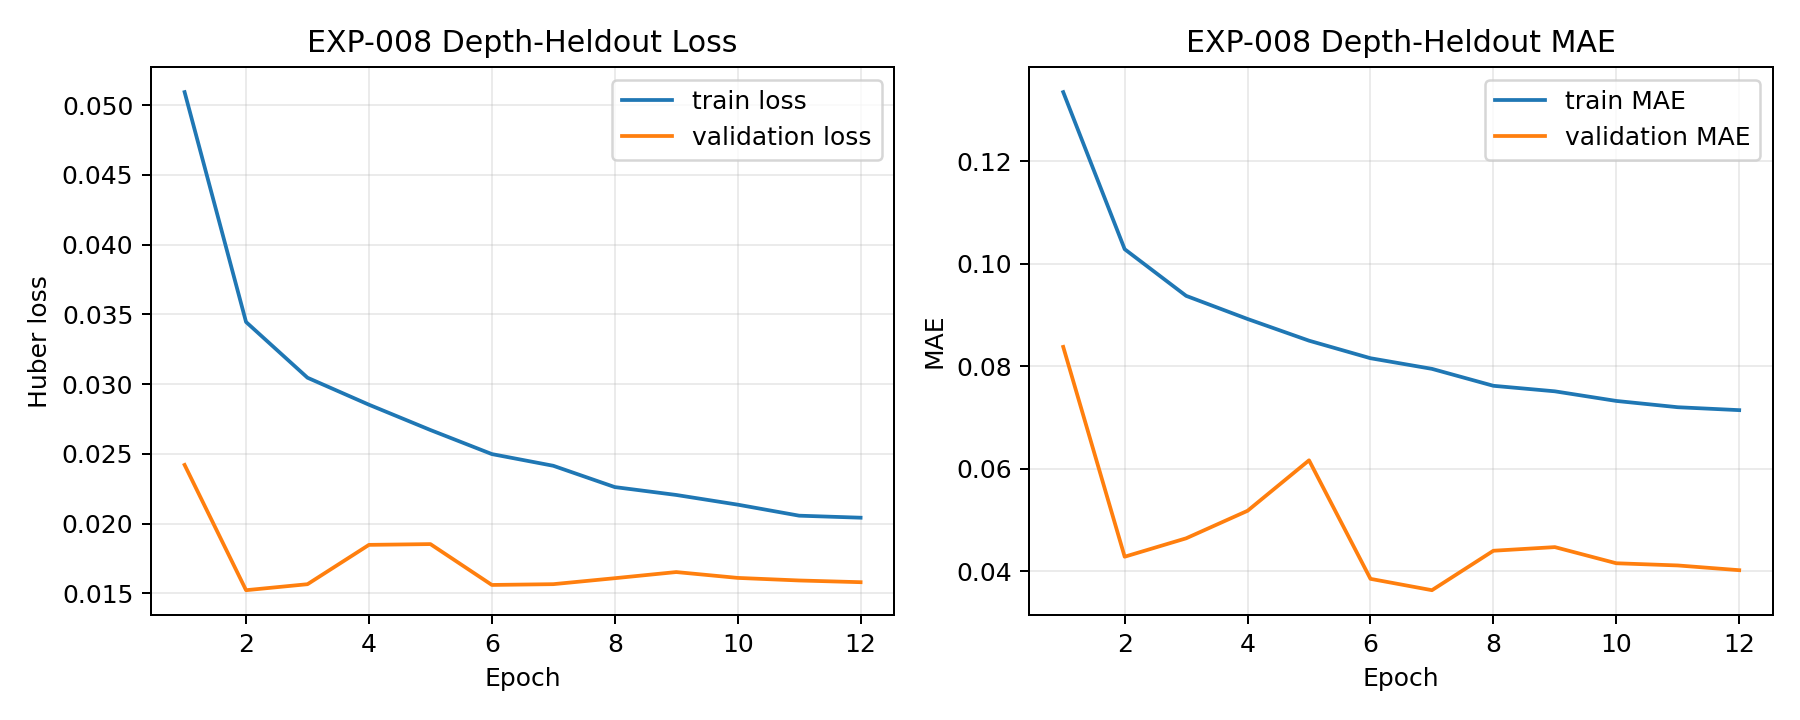
\includegraphics[width=0.94\textwidth]{figures/revision/exp3_training_curve.png}
  \caption{实验三训练损失与验证损失曲线}
  \label{fig:exp3-training}
\end{figure}

\subsection{验证集与测试集指标}

实验三的验证集和测试集指标见表 \ref{tab:exp3-metrics}。测试集包含 423 个样本、888300 个标签元素。测试 $R^2=0.106634$，说明模型相对测试标签均值只能解释有限比例的方差；Pearson 系数 0.351950、Spearman 系数 0.480519，表现为中等偏弱的正相关。该结果支持“存在一定可学习性”，不支持“高精度反演”。

\begin{table}[htbp]
  \centering
  \caption{实验三的验证集与测试集整体指标}
  \label{tab:exp3-metrics}
  \begin{tabular}{lrrrrrr}
    \toprule
    集合 & MAE & RMSE & $R^2$ & Pearson & Spearman & $n$ \\
    \midrule
    验证集 & 0.042817 & 0.187167 & 0.010882 & 0.200575 & 0.266137 & 416 \\
    测试集 & 0.079025 & 0.277019 & 0.106634 & 0.351950 & 0.480519 & 423 \\
    \bottomrule
  \end{tabular}
\end{table}

预测与真实值散点见图 \ref{fig:exp3-scatter}。大量标签元素聚集在零值附近，非零标签分布更分散。模型能够产生与真实值同向变化的响应，但对较大目标的覆盖不足；这与较低的 $R^2$ 和有限相关性相一致。

\begin{figure}[htbp]
  \centering
  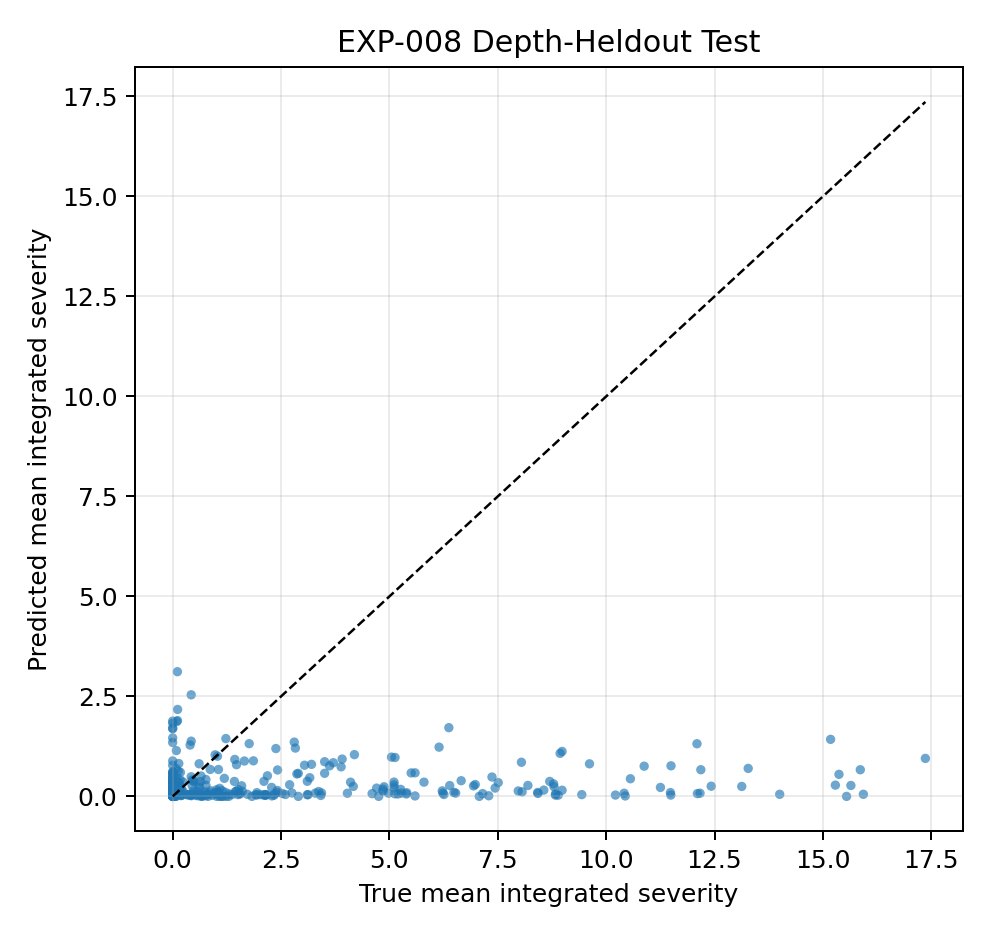
\includegraphics[width=0.72\textwidth]{figures/revision/exp3_prediction_scatter.png}
  \caption{实验三测试集预测值与真实值散点}
  \label{fig:exp3-scatter}
\end{figure}

\section{基线比较}

表 \ref{tab:exp3-baseline} 和图 \ref{fig:exp3-baseline} 比较模型与三类简单基线。零值基线将全部 $70\times30$ 标签预测为 0；训练集均值和中位数基线分别用训练标签的逐元素统计量预测测试样本。

\begin{table}[htbp]
  \centering
  \caption{实验三与简单基线的测试集比较}
  \label{tab:exp3-baseline}
  \begin{tabular}{lrrr}
    \toprule
    方法 & MAE & RMSE & $R^2$ \\
    \midrule
    本文模型 & 0.079025 & 0.277019 & 0.106634 \\
    零值基线 & \textbf{0.069751} & 0.301272 & -0.056638 \\
    训练集均值基线 & 0.142358 & 0.316129 & -0.163426 \\
    训练集中位数基线 & 0.119024 & 0.278963 & 0.094049 \\
    \bottomrule
  \end{tabular}
\end{table}

\begin{figure}[htbp]
  \centering
  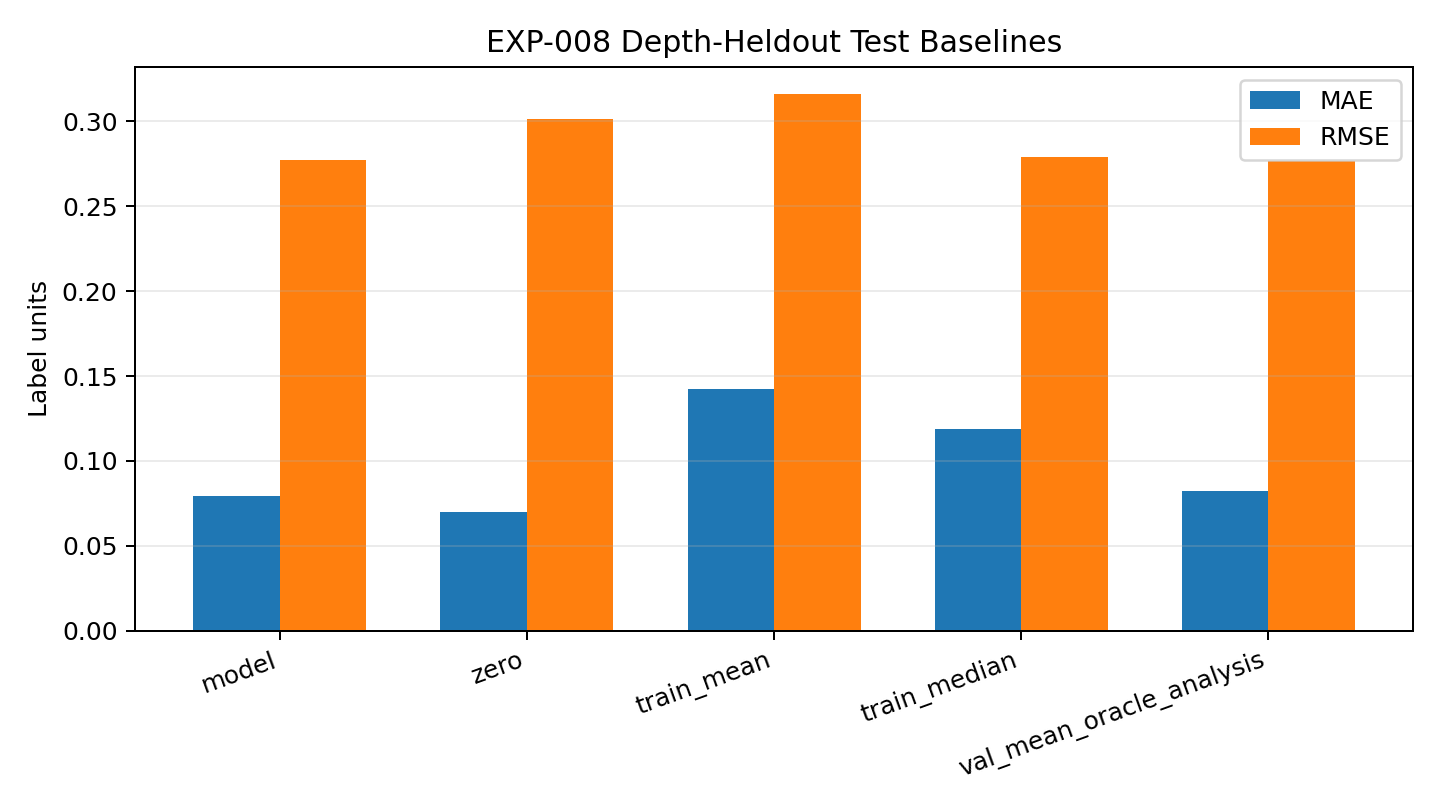
\includegraphics[width=0.91\textwidth]{figures/revision/exp3_baseline_comparison.png}
  \caption{实验三模型与简单基线的 MAE、RMSE 和 $R^2$}
  \label{fig:exp3-baseline}
\end{figure}

比较结果具有指标依赖性。模型的 MAE 没有优于零值基线，说明标签稀疏时“全部预测为零”可获得较低平均绝对误差；但模型的 RMSE 和 $R^2$ 优于零值基线，表明模型对部分非零结构的预测减少了较大平方误差。模型在三项指标上均优于训练集均值基线。与训练集中位数基线相比，模型 RMSE 只改善 0.001944，差距很小；$R^2$ 略高，MAE 较低。因而不存在“所有指标全面领先”的结论。

标签元素的绝对误差中有较高比例集中在零附近，使 MAE 对稀疏区域权重较大。RMSE 对大误差更敏感，$R^2$ 又以测试集方差为参照，三者回答的问题不同。本文保留全部指标，不选择性报告对模型有利的结果。

\section{FFT 系数误差}

图 \ref{fig:exp3-coeff} 给出 $k=0$--29 各系数 MAE。测试集中 $k=0$--4 的平均 MAE 为 0.131411；按既有汇总口径，$k=0$--5 的 MAE 为 0.128785，而 $k=15$--29 的 MAE 为 0.050184。低阶系数包括周向总量和较大尺度结构，其目标幅值总体较大，因此绝对误差也较高。

\begin{figure}[htbp]
  \centering
  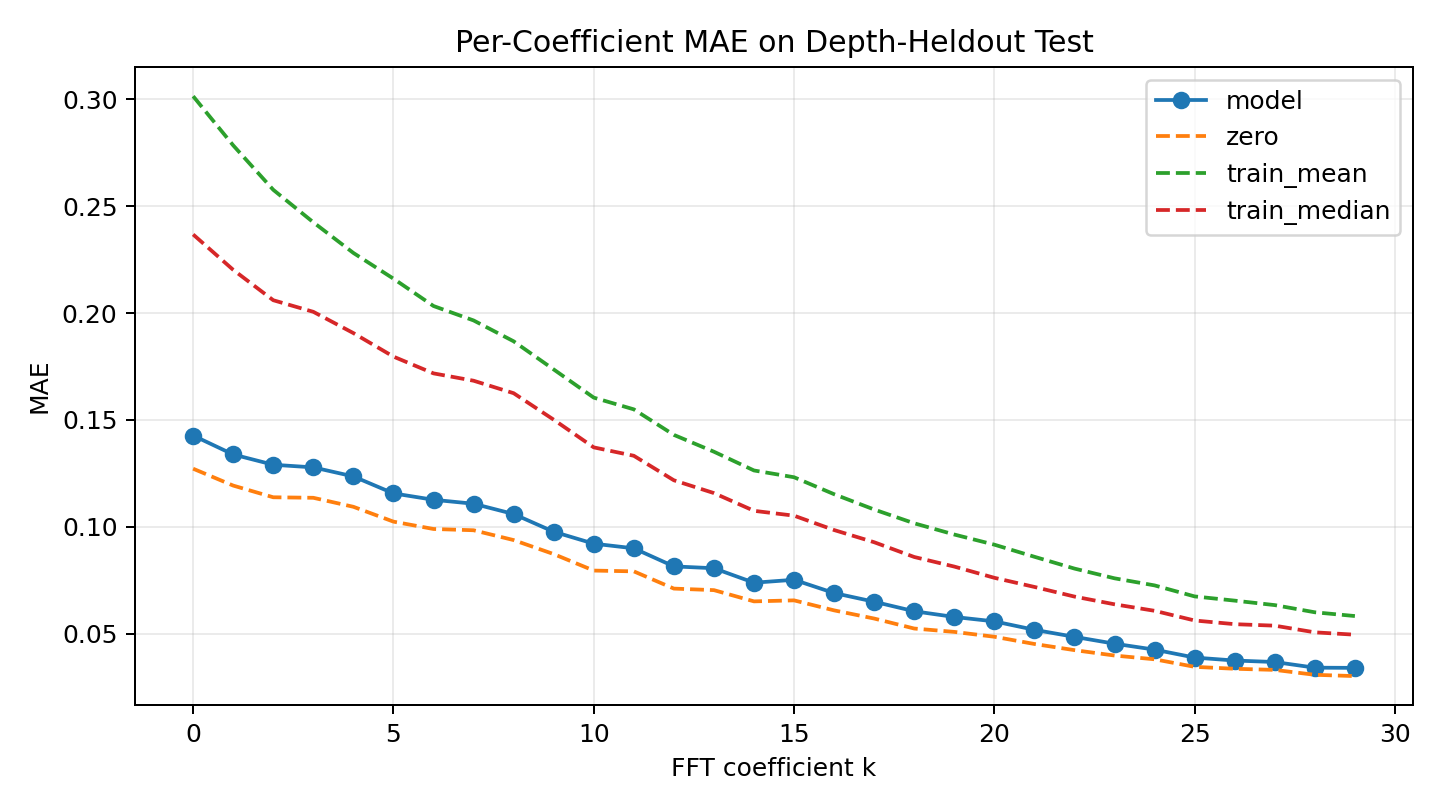
\includegraphics[width=0.93\textwidth]{figures/revision/exp3_coefficient_mae.png}
  \caption{实验三各方位 FFT 系数的测试 MAE}
  \label{fig:exp3-coeff}
\end{figure}

高阶系数 MAE 较小不能直接解释为“高频结构更容易学习”。当目标系数本身接近零时，即使模型忽略其变化，绝对误差也可能较小。因而需要结合目标幅值、归一化误差和结构重构共同判断。现有证据只支持低阶系数是总体绝对误差的重要组成部分。

\section{高严重度样本误差}

为观察标签分布，将测试样本按真实平均积分严重度分组。423 个测试样本中，177 个为零，171 个位于 $(0,5)$，75 个位于 $[5,20)$，没有样本达到 20 以上。该分布说明测试集同时具有大量零样本和有限的较高严重度样本。

图 \ref{fig:exp3-lowfreq} 比较低频摘要的真实值与预测值。误差较大的高严重度样本中，预测通常低于真实峰值，结果提示模型可能存在向样本中心收缩的倾向。可能原因包括较高严重度样本数量有限、ReLU 多输出回归的稀疏目标、损失由大量低值元素主导以及同井深度区间分布变化。现有实验没有逐项验证这些机制，因此只能将其列为可能因素。

\begin{figure}[htbp]
  \centering
  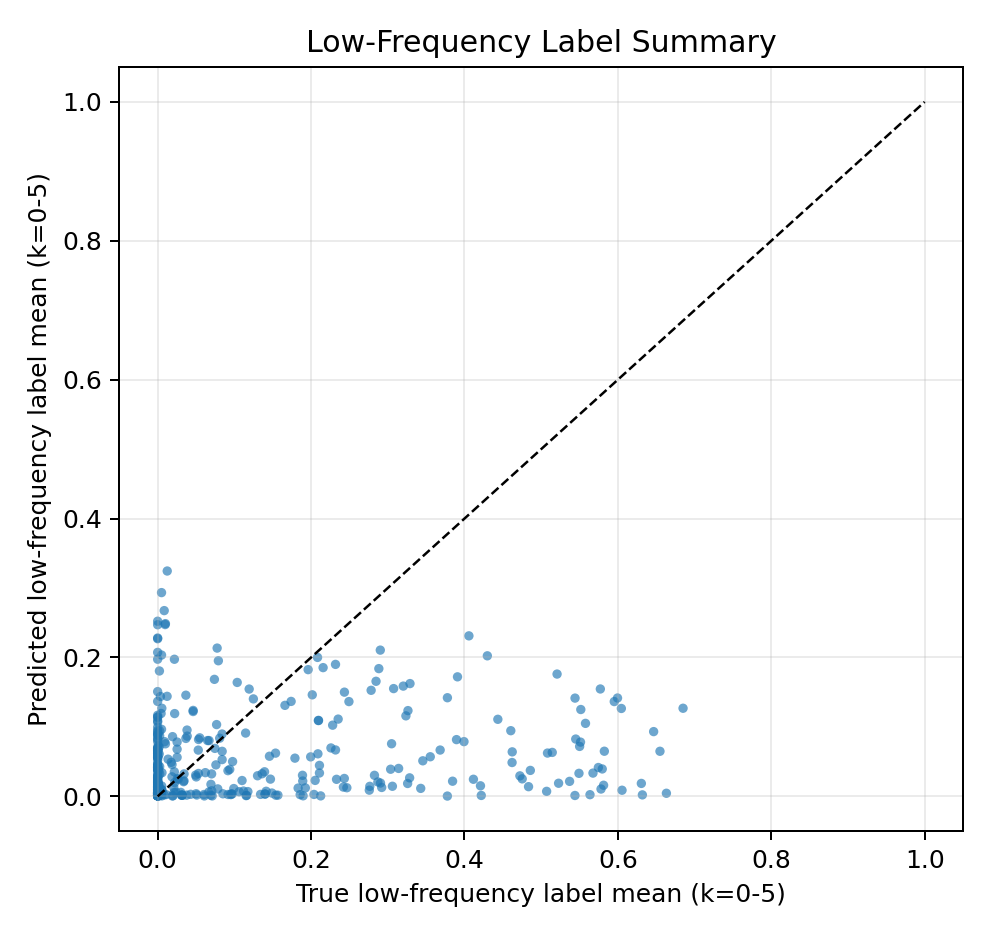
\includegraphics[width=0.72\textwidth]{figures/revision/exp3_lowfreq_summary.png}
  \caption{实验三低频结构摘要的真实值与预测值比较}
  \label{fig:exp3-lowfreq}
\end{figure}

测试残差分布见图 \ref{fig:exp3-error}。分布集中于零附近但存在长尾，与 RMSE 高于 MAE 所反映的少量较大误差一致。对固井质量研究而言，较高严重度样本更值得关注；因此，总体平均指标不能替代分组误差分析。

\begin{figure}[htbp]
  \centering
  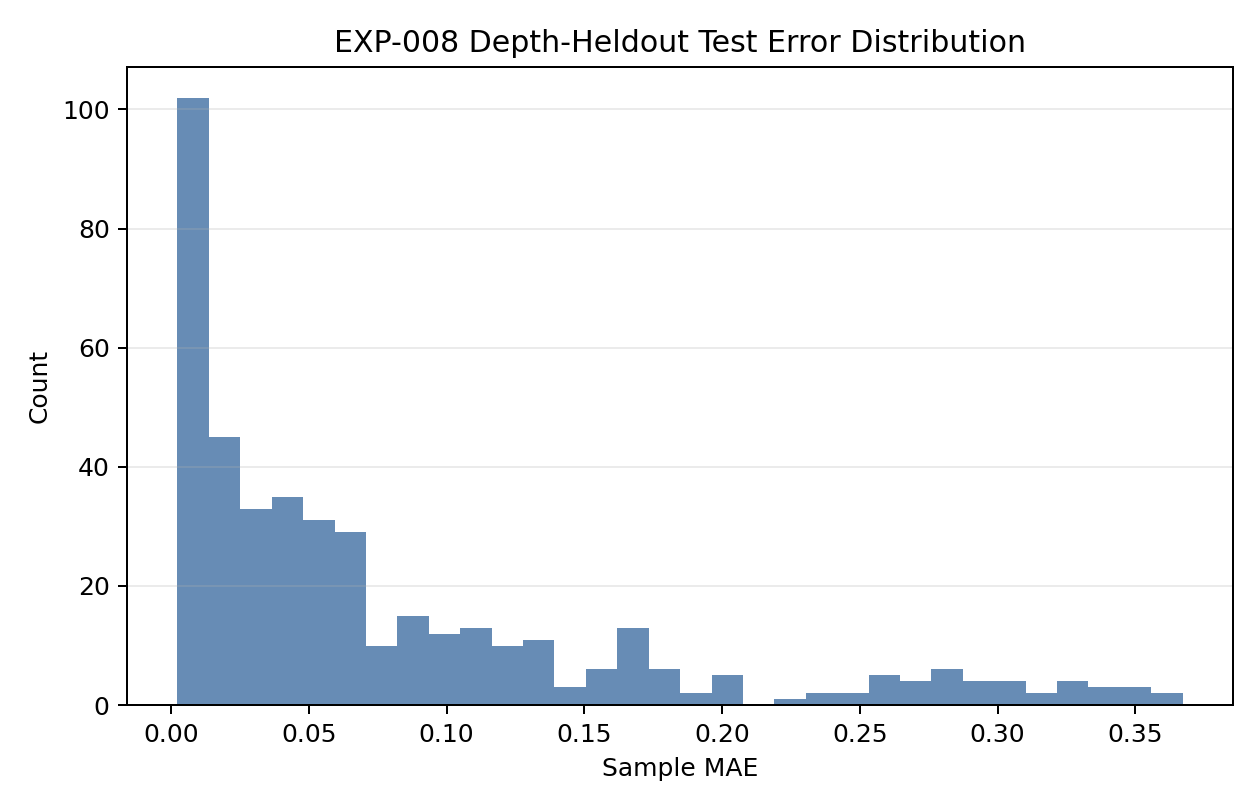
\includegraphics[width=0.88\textwidth]{figures/revision/exp3_error_distribution.png}
  \caption{实验三测试集标签元素误差分布}
  \label{fig:exp3-error}
\end{figure}

\section{实验二对照结果}

实验二使用一维窜槽占比标签，将每个深度位置的 180 个周向采样压缩为一个占比。输出维度降低后，模型不再需要预测方位结构，但仍要从 XSI 时频响应迁移到隔离测试井段。测试结果见表 \ref{tab:exp2-metrics}。

\begin{table}[htbp]
  \centering
  \caption{实验二的单井深度区间隔离测试指标}
  \label{tab:exp2-metrics}
  \begin{tabular}{lr}
    \toprule
    指标 & 数值 \\
    \midrule
    MAE & 0.811672 \\
    RMSE & 2.832056 \\
    $R^2$ & -0.011278 \\
    Pearson & 0.198048 \\
    Spearman & 0.413335 \\
    \bottomrule
  \end{tabular}
\end{table}

负 $R^2$ 表明实验二在平方误差意义下未优于以测试均值为参照的常数预测。Pearson 相关较弱，Spearman 为正，说明预测排序中仍有部分信息，但幅值拟合不足。该结果说明，简单降低标签维度并未消除深度区间迁移困难。一维标签对照的价值在于揭示方位平均造成的信息损失，而不是提供比实验三更强的性能结论。

\section{实验一结果的使用边界}

实验一的高验证 AUC 仅在随机样本划分条件下成立。与实验二、实验三的深度区间隔离结果相比，它说明 CWT 输入中存在与 CAST 派生标签相关的可学习信号，却不能回答该信号能否稳定迁移到未见连续井段。本文不把二分类准确率与回归 MAE、$R^2$ 直接比较，也不以实验一替代主实验的严格验证。

\section{Grad-CAM 可解释性分析的证据边界}

Grad-CAM 的方法定义和解释边界已在第 3 章给出\cite{Selvaraju2017GradCAM}。现有候选图件可部分追溯到早期 FFT 回归分析脚本，但无法把每张图唯一对应到生成时的模型 checkpoint、训练运行、样本深度和数据划分；分析脚本还将全部回归输出之和作为标量目标，不能据此解释某一特定深度位置或 FFT 系数。因此，这些图件不满足本文主要实验的结果准入条件，本章不插入热图，也不声称已经完成单井深度区间隔离模型的 Grad-CAM 验证。

这一取舍不影响前述预测指标和误差分析。后续只有在模型版本、划分、checkpoint、样本深度、目标输出和卷积层同时可追溯时，才适合比较不同样本的时频响应区域；即使证据链完整，热图也只能解释为针对特定预测的梯度加权特征响应，不能作为物理因果证据。

\section{本章小结}

本章在相同单井深度区间隔离划分下比较了两种回归标签，并以随机样本划分二分类作为先导验证。实验三测试 MAE 为 0.079025、RMSE 为 0.277019、$R^2$ 为 0.106634，相关性为中等偏弱，支持有限可学习性而非高精度结论。模型在 RMSE 和 $R^2$ 上优于零值基线，却未在 MAE 上占优；与训练集中位数基线的 RMSE 接近。低阶 FFT 系数和较高严重度样本构成主要误差来源。实验二降低输出维度后 $R^2$ 仍为负，说明深度区间迁移并未因标签简化而解决。来源链不完整的 Grad-CAM 图件未作为实验结果使用。

\chapter{讨\hspace{6pt}论}

\section{与现有固井评价方法的关系}

井完整性研究强调套管和水泥屏障需要结合服役场景进行评价\cite{Kiran2017WellIntegrityReview,Bai2016WellIntegrityReview}。传统 CBL 和 VDL 通过套管波幅度、衰减和波形连续性评价胶结状态，其优势是技术成熟、解释路径清晰，但结果受套管、水泥、工具和地层条件共同影响\cite{Pardue1963CementBond,Wang2016AcousticCementMethods}。周向分区和方位阵列工具通过增加周向敏感单元改善局部缺陷识别\cite{Bigelow1990SegmentedBond,Lu2014AzimuthalAcoustic,Zuo2020AzimuthCement}。超声脉冲回波和周向成像则能提供更直观的套管后介质图像\cite{Froelich1982CementEvaluation,VanKuijk2005UltrasonicImager}。本文并不替代这些物理测量，而是研究在已有 XSI 和 CAST 资料之间建立可追溯的统计映射。

与直接方位成像方法不同，本文没有可靠的共同绝对方位零点。方位声学文献中，接收阵列的方向解释建立在工具几何和参考方向已知的条件上\cite{Che2014PhasedArcReception,Che2017AzimuthalReceiver}。本文主要实验井段整体接近直井，Inclination 中位数约为 $0.4705^\circ$，Relative Bearing 又存在频繁跳变；Inclination 仅描述井斜大小，不能替代绕工具轴的旋转角。本文因而不使用绝对方位位置作为监督，而以 FFT 幅值保留环向结构的频率组成，使同一结构在未知循环移位下具有相同标签。其价值是降低未知方位移位造成的监督不一致，而不是提高仪器方位分辨率或恢复窜槽的绝对方位。

\section{标签设计的价值与信息损失}

一维窜槽占比标签对方位零点完全不敏感，但把连续宽通道、多个离散异常和不同幅值分布压缩为相同占比。FFT 幅值标签保留周向总量和不同尺度的周期结构，因此比单一占比包含更多结构信息。离散傅里叶平移关系给出了其循环平移不变性的数学依据，傅里叶描述子研究也说明频域幅值可用于表达不依赖起点的形状特征\cite{Zahn1972FourierDescriptors,Persoon1977FourierDescriptors,Kuhl1982EllipticFourier}。

该设计同时存在不可逆损失。舍弃相位后，模型无法恢复窜槽位于哪个绝对方位；不同序列还可能具有相同幅值谱。只保留前 30 个系数又进一步削弱细尺度周向变化。因此，本文题目中的“结构特征反演”应理解为对旋转不变频谱特征的预测，不应解释为重构完整 CAST 图像或恢复绝对窜槽位置。

阈值 $2.5~\mathrm{MRayl}$ 是哈里伯顿公司在本项目 CAST 成像解释中采用的项目约定，不是本文提出或通过优化得到的普适行业标准。全井 $Z_c$ 中的 14 个负值缺乏合理物理意义，历史代码没有显式屏蔽；但位置复核表明它们全部位于本文目标井段之外，目标插值网格中没有负值，因而未进入一维占比、严重度或 FFT 标签以及模型训练、验证和测试。因此，这些负值不影响本文主要实验结果，而阈值选择、参考工具测量和频谱变换仍会共同影响派生标签效度。实验结果描述的是对该派生表征的学习程度，而不是对地下水泥环真实几何的直接测量精度。

\section{CWT 表征与网络骨干的作用}

CWT 将非平稳声波映射为局部时间--频率表示，较整体频谱保留到达时间。声波测井时频小波研究和水泥评价迁移学习应用均表明，这类表示适合处理波形中随时间变化的频率成分\cite{Saito1997WaveletAcoustic,Abdollahian2024TransferCement}。本文实验一也表明，在随机样本划分下，CWT 输入包含与 CAST 派生类别相关的可学习信息。

EfficientNetV2B0 在本文中只是特征提取骨干。其训练效率和结构缩放特点来自原始方法\cite{Tan2021EfficientNetV2}，不能作为本文网络创新。当前数据量、输出维度和早期过拟合现象表明，单纯增加网络容量未必改善深度区间迁移。与水泥评价分类、固井参数预测和声波日志重构研究相比\cite{Viggen2020AutomaticCement,Liu2025WideDeepCement,Wang2023ExplainableSonic}，本文的输入、标签和验证目标均不同，不能直接比较准确率或误差数值。

\section{单井深度区间隔离结果的解释}

实验三测试 $R^2=0.106634$，Pearson 为 0.351950，Spearman 为 0.480519。正相关和正 $R^2$ 表明模型在未见连续深度区间中保留了一部分与标签变化相关的信息，但解释方差有限。验证损失第 2 轮达到最佳，说明模型很快拟合主要模式，之后没有获得稳定的验证改善。

深度区间隔离减少了相邻样本直接混入不同集合的风险。结构化数据验证研究表明，分块验证通常比随机划分更能反映迁移到新空间或时间区间的误差\cite{Roberts2017CrossValidation,Ploton2020SpatialValidation}。但本文仍只有单井、单接收环数据。不同井之间可能存在套管规格、地层、井液、仪器增益、姿态和标签分布差异，单井深度隔离不能替代跨井验证，也不能据此判断工业部署条件下的稳定性。

\section{零值基线与稀疏标签}

实验三的零值基线 MAE 为 0.069751，低于模型的 0.079025；模型则在 RMSE 和 $R^2$ 上优于零值基线。该差异来自指标对误差分布的权重不同：MAE 对每个元素等权，大量零或近零标签使全零预测占优；RMSE 对少量大误差更敏感，模型对部分非零结构的预测可以降低平方误差。

因此，“模型是否优于基线”没有脱离指标的唯一答案。本文只能陈述：模型对非零结构显示了一定学习能力，但没有在平均绝对误差上击败最简单的稀疏标签基线。训练集中位数基线的 RMSE 与模型非常接近，也说明总体结果仍受标签中心分布强烈约束。后续可考虑非零区域指标、分严重度评价或与工程风险相关的代价函数，但在没有新增实验前不能把这些设想写成已验证改进。

\section{低频误差与高严重度低估}

低阶 FFT 系数承载周向总量和大尺度结构，其目标幅值较大，测试绝对误差也高。高阶系数 MAE 较小主要可能来自目标幅值较小，而不一定表示模型更容易学习细尺度结构。后续分析应同时报告归一化误差、目标能量和重构差异，避免只依据绝对 MAE 判断不同频率的难度。

测试样本中没有平均积分严重度超过 20 的样本，5--20 区间仅 75 个。较高严重度样本的预测峰值普遍不足，提示模型可能向常见低值收缩。样本不平衡、Huber 损失对大误差的线性增长、高维输出中的稀疏元素和区间分布变化都可能参与这一现象，但本研究没有设计消融实验区分这些因素。该问题直接限制了模型在高风险井段筛查中的用途。

\section{Grad-CAM 的解释边界}

Grad-CAM 依据指定目标输出对卷积特征图的梯度生成粗粒度响应区域\cite{Selvaraju2017GradCAM}。对于本文的多输出回归，不同深度位置、不同 FFT 系数或不同系数组合对应不同目标，热图必须随目标定义一起报告。热区只能说明该预测在局部线性梯度意义下对某些时频区域敏感，不能解释为网络参数，也不能证明真实物理因果。

现有候选热图只能部分追溯到早期 FFT 回归分析，无法同时确定每张图生成时的 checkpoint、训练运行、样本深度和数据划分，且其标量目标是全部回归输出之和。因此，本文没有把这些图用于实验三解释。后续若建立完整的可追溯分析，应先固定测试样本和目标系数，再比较不同误差样本、接收通道和声波到达时窗；即使完成这些步骤，结论仍应限定为模型响应与物理时窗之间的空间一致性，而非机理证明。

\section{研究有效性威胁}

本文的主要有效性威胁包括：CAST 的 $2.5~\mathrm{MRayl}$ 阈值仅适用于本项目数据约定；Relative Bearing 的正式参考方向和 CAST 零点不能形成与 XSI 唯一对应的共同方位基准；XSI 波形存在少量有符号 24 位端点削顶，历史预处理没有专门恢复；严格验证只覆盖单井第 3 接收环；较高严重度样本有限；输出幅值谱不能恢复绝对方位。XSI 端点数量极少，经项目数据核查，其对总体实验结果的影响可以忽略，但仍属于输入数据质量现象。CAST 全井 14 个负值因位于目标井段之外而没有进入本文标签，不构成主要实验指标的不确定来源。上述限制分别影响标签解释、输入质量、外部效度和结论范围。

上述问题并不否定当前实验的研究价值，但决定了结果应被表述为方位失配条件下的一次可追溯方法验证。只有在补充工具姿态元数据、跨井数据和更完整的标签质量控制后，才能进一步讨论绝对方位、跨井稳定性和工程应用。

\section{本章小结}

本章将本文方法置于传统声幅、方位阵列、超声成像和数据驱动固井评价的技术脉络中。FFT 幅值标签在不使用绝对方位位置的同时保留环向结构的频率组成，但以丢失相位、绝对方位和部分细尺度结构为代价；CWT 与 EfficientNetV2B0 提供了实现路径，而非结论本身。单井深度区间隔离结果显示有限可学习性，同时暴露了零值基线 MAE、低阶系数误差、高严重度低估和跨井证据缺失等限制。

\chapter{结论与展望}

\section{主要结论}

本文围绕 XSI 声波测井与 CAST 超声成像测井之间的方位失配问题，研究了基于 CWT 时频特征和 CAST 弱监督标签的水泥窜槽结构特征反演方法。主要结论如下：

\begin{enumerate}
  \item 针对 XSI 与 CAST 直接方位点对点监督不可靠的问题，本文构造了一维 percentage label 和 FFT severity magnitude label 两类弱监督标签。其中，FFT magnitude 标签通过丢弃相位降低对绝对方位匹配的依赖，更适合作为本文方法主线。
  \item 在 \texttt{array\_03} 单井 depth-heldout 条件下，EXP-008 取得 Test MAE 0.079025、RMSE 0.277019、R2 0.106634、Pearson 0.351950 和 Spearman 0.480519。该结果说明 FFT severity magnitude 标签具有一定可学习性，但不构成多井泛化证明。
  \item EXP-008 优于 train-mean 和 train-median baseline 的 MAE/RMSE/R2，并优于 zero baseline 的 RMSE/R2；但其 MAE 未优于 zero baseline。因此，本文只能将其表述为 metric-qualified learnability，而不能写成全面优于简单基线。
  \item EXP-007 一维 percentage label 在同一单井 depth-heldout 设置下可训练，但 Test R2 为 -0.011278，且 MAE 同样未优于 zero baseline。该结果支持其作为 fallback/limitation comparison，而不替代 EXP-008 主线。
  \item EXP-006 二分类 baseline 仅在 random split 设置下说明 CWT 与 CAST 派生窜槽标签存在可学习关系，不作为最终 depth-heldout 性能证据。
\end{enumerate}

\section{创新点总结}

本文的主要创新点体现在以下方面：

\begin{enumerate}
  \item 从方位失配问题出发，将 CAST Zc 图像转化为弱监督标签，避免直接依赖不可靠的 XSI--CAST 点对点方位匹配。
  \item 提出并验证 severity map 到方位向 FFT magnitude 标签的主线方法，用频域幅值表征降低对环向旋转相位的依赖。
  \item 将 XSI 全波列 CWT 时频图与 EfficientNetV2B0 回归模型结合，用于学习 CAST 派生窜槽结构特征。
  \item 在证据整理中明确区分 random split exploratory evidence 与 single-well depth-heldout evidence，避免将相邻深度泄漏风险下的旧指标写成最终泛化性能。
\end{enumerate}

\section{不足与展望}

本文仍存在明显限制。首先，最终 depth-heldout 实验仅覆盖 \texttt{array\_03} 单井，无法代表多井泛化。其次，EXP-008 和 EXP-007 均未在 MAE 上优于 zero baseline，说明稀疏标签下的评价体系和模型目标仍需改进。再次，EXP-008 对低频 FFT 系数和高严重度样本存在较大误差，高风险窜槽段低估问题需要进一步研究。最后，Grad-CAM 等可解释性证据目前只能作为定性分析，尚不能构成物理因果证明。

后续工作可从四个方向展开：一是增加多井或跨井 depth-heldout 验证，评估方法在不同井段和工况下的稳定性；二是设计面向非零区域和高严重度样本的评价指标与损失函数；三是针对低频 FFT 系数进行更细粒度的误差建模；四是结合声学机理和批量可解释性统计，进一步分析模型关注区域与物理响应之间的关系。


% TODO: 补齐真实文献条目后，可改用 \thesisbibliography{refs/references}。
\begin{thesisthebibliography}
% \bibitem{todo} TODO: 在正式提交前补充声波测井、CAST、CWT、EfficientNet、Grad-CAM 等真实文献。
\end{thesisthebibliography}

\thesisappendix
\chapter{旧项目实验路线补充说明}

\section{失败路线与附录定位}

旧项目中曾尝试多条方法路线，包括 SE-ResNet 方位匹配、GAN 或 two-channel binary FFT label、dual-channel metadata fusion、eccentricity pre-correction、sample weights 与 asymmetric loss 等。这些路线没有形成稳定优于 EXP-008 主线的最终证据，因此不作为正文主线展开。

\section{SE-ResNet 方位匹配路线}

SE-ResNet 路线尝试直接利用声波通道与 CAST 方位结构之间的对应关系。但由于 XSI 与 CAST 的相对方位参考不可靠，直接方位匹配路线容易受到标签错配影响。本文仅将其作为方法探索背景，不作为最终性能证据。

\section{dual-channel metadata fusion}

dual-channel metadata fusion 尝试将声波 CWT 输入与偏心或元数据信息联合输入模型。旧证据显示该路线未能学习到稳定有效特征，因此不进入正文主线。

\section{eccentricity pre-correction}

eccentricity pre-correction 试图利用偏心信息对波形或特征进行预校正。最终证据表明该路线效果较差，不能支撑论文主结果。本文将其用于说明为什么最终转向弱监督标签工程，而不是作为新的实验主线。

\section{sample weights 与 asymmetric loss}

样本权重和非对称损失曾用于尝试缓解高严重度样本预测不足问题。远程分支核验显示该路线效果很差，适合作为 failed attempt 或附录说明，不应在正文中写成有效改进。

\section{GAN 与 two-channel binary FFT label}

GAN 或 two-channel binary FFT label 路线证据不足，且与最终 single-well depth-heldout 主线不一致。本文不继续训练该路线，也不将其作为正文实验结果。

\section{附录小结}

上述失败路线的价值在于说明本文技术取舍：直接方位匹配、元数据融合和偏心预校正均未形成稳定证据；最终采用 CWT-EfficientNet 与 FFT severity magnitude 弱监督标签，是在旧项目探索基础上形成的更适合论文主线的方案。


\thesisacknowledgement
TODO：致谢内容由作者根据实际情况补充。

\end{document}
